\documentclass[UTF8]{ctexart}
\usepackage{amsmath}
\usepackage{amsfonts}
\usepackage{amssymb}
\usepackage{graphicx}
\usepackage{hyperref}
\usepackage{float}
\usepackage{caption}
\usepackage{subfig}
\usepackage{bm}
\usepackage{mathrsfs}
\usepackage{latexsym}
\usepackage{euscript}
\usepackage{esint}
\usepackage{blindtext}
\renewcommand\thesection{\Roman{section}}

\hypersetup{colorlinks=true,linkcolor=black}

% Title Page
\title{$ \gamma $射线的吸收与物质吸收系数$ \mu $的测定实验报告}
\author{17377306\ 马晓天}
\RequirePackage[a4paper]{geometry}
\geometry{
	textwidth=138mm,
	textheight=215mm,
	left=27mm,
	right=27mm,
	top=25.4mm, 
	bottom=25.4mm,
	headheight=2.17cm,
	headsep=4mm,
	footskip=12mm,
	heightrounded,
}


\begin{document}
\maketitle

\thispagestyle{empty}
\section{数据分析}
实验条件为：$^{60}$Co放射源，NaI(TI)探测器(SG1121(4040))，游标卡尺(1/50mm分度)，高压电源为500V，放大器放大倍数为$ 0.9\times50=45 $，定标器阈值为0.31V，采用铁片测量。
实验原始数据为:
\begin{table}[H]
	\centering
	\caption{Fe片的厚度测量数据}
	\begin{tabular}{ccccccc}
		\hline
		$ i $ & 1 & 2 & 3 & 4 & 5 & 6\\
		\hline
		$ t_{1} $/cm & 0.206 & 0.210 & 0.206 & 0.208 & 0.200 & 0.202\\
		$ t_{2} $/cm & 0.202  & 0.208  & 0.216  & 0.210  & 0.202  & 0.210\\
		$ t_{3} $/cm & 0.200  & 0.216  & 0.206  & 0.204  & 0.204  & 0.204\\
		$ \overline{t}$/cm  & 0.203  & 0.211  & 0.209  & 0.207  & 0.202  & 0.205\\
		$ u(\overline{t}) $/cm & 0.003  & 0.004  & 0.006  & 0.003  & 0.002  & 0.004\\
		\hline
	\end{tabular}
\end{table}
其中$ i $代表第$ i $块铁片，实验中将六块铁片编号，分别测量它们的厚度($t_1/t_2/t_3$)，叠加得到各次实验的实际铁片厚度(表2中的$ t $)，$ u(\overline{t})$代表$ \overline{t} $的不确定度。
\begin{table}[H]
	\centering
	\caption{吸收系数测量数据}
	\begin{tabular}{cccccccc}
		\hline
		$ t $/cm & 0  & 0.203  & 0.414  & 0.623  & 0.831  & 1.033  & 1.238\\
		\hline
		$ u(t)$/cm & 0  & 0.003  & 0.005  & 0.008  & 0.009  & 0.009  & 0.010\\
		$ t_{\rm s} $/s & 50 & 60 & 60 & 60 & 60 & 60 & 60\\
		$ N_{\rm s} $ & 19791 & 23311 & 22916 & 22363 & 21765 & 21431 & 21101\\
		$ n_{\rm s}/\rm s^{-1} $ & 395.82  & 388.52  & 381.93  & 372.72  & 362.75  & 357.18  & 351.68 \\
		$ n_{0}/\rm s^{-1}$ & 228.13  & 220.83  & 214.24  & 205.03  & 195.06  & 189.49  & 183.99\\
		$ \sigma_{n_{0}}/\rm s^{-1} $ & 3.10  & 2.86  & 2.84  & 2.81  & 2.78  & 2.76  & 2.75\\
		$ \ln n_{0}$  & 5.430  & 5.397  & 5.367  & 5.323  & 5.273  & 5.244  & 5.215\\
		$ \sigma_{\ln n_{0}} $ & 0.014  & 0.013  & 0.013  & 0.014  & 0.014  & 0.015  & 0.015\\
		\hline
	\end{tabular}
\end{table}
其中$ t_{\rm s} $为测量时间，$ N_{\rm s} $为测量计数，$ n_{\rm s} $为计数率，$ n_0=n_{\rm s}-n_{\rm b} $为净计数率，$ \sigma_{n_{0}} $和$ \sigma_{\ln n_{0}} $为标准误差。环境本底测量时间$ t_{\rm b}=100\rm s $，计数$ N_{\rm b}=16769 $，计数率$ n_{\rm b}=167.69\rm s^{-1} $，标准误差$ \sigma_{n_{\rm b}}=1.29\rm s^{-1}$。
\subsection*{Fe片吸收系数的测定}
$ \gamma $射线强度随物质厚度的衰减服从指数规律，即：
\begin{equation}
I=I_{0} e^{-\sigma_{\rm r} N t}=I_{0} e^{-\mu t}
\end{equation}
其中，$ I_{0}$、$ I $分别是穿过物质前、后的$ \gamma $射线强度，$t$是$ \gamma $射线穿过的物质的厚度(单位为cm)，$ \sigma_{\rm r} $是光电、康普顿、电子对三种效应截面之和，N是吸收物质单位体积中的原子数，$ \mu $是物质的线性吸收系数($ \mu=\sigma_{\rm r}N $，单位为$\rm cm^{-1} $)。由于在相同的实验条件下，某一时刻的计数率$ n $总与该时刻的$ \gamma $射线强度$ I $成正比，取对数得：
\begin{equation}
\ln n_{0}=-\mu t+\ln n_{\rm I_{0}}
\end{equation}
采用如下函数族进行拟合：
\begin{equation}
y=a+b*x
\end{equation}
其中，$ y=\ln n_{0} $，$ x=t $，拟合得到：
\begin{equation*}
a=5.434\pm0.009,b=-0.181\pm0.013,R^2=0.9943
\end{equation*}
比较式(2)(3)可得：
\begin{equation}
\mu=-b=0.18\pm0.01\rm cm^{-1}
\end{equation}
拟合效果如图1：
\begin{figure}[H]
	\centering
	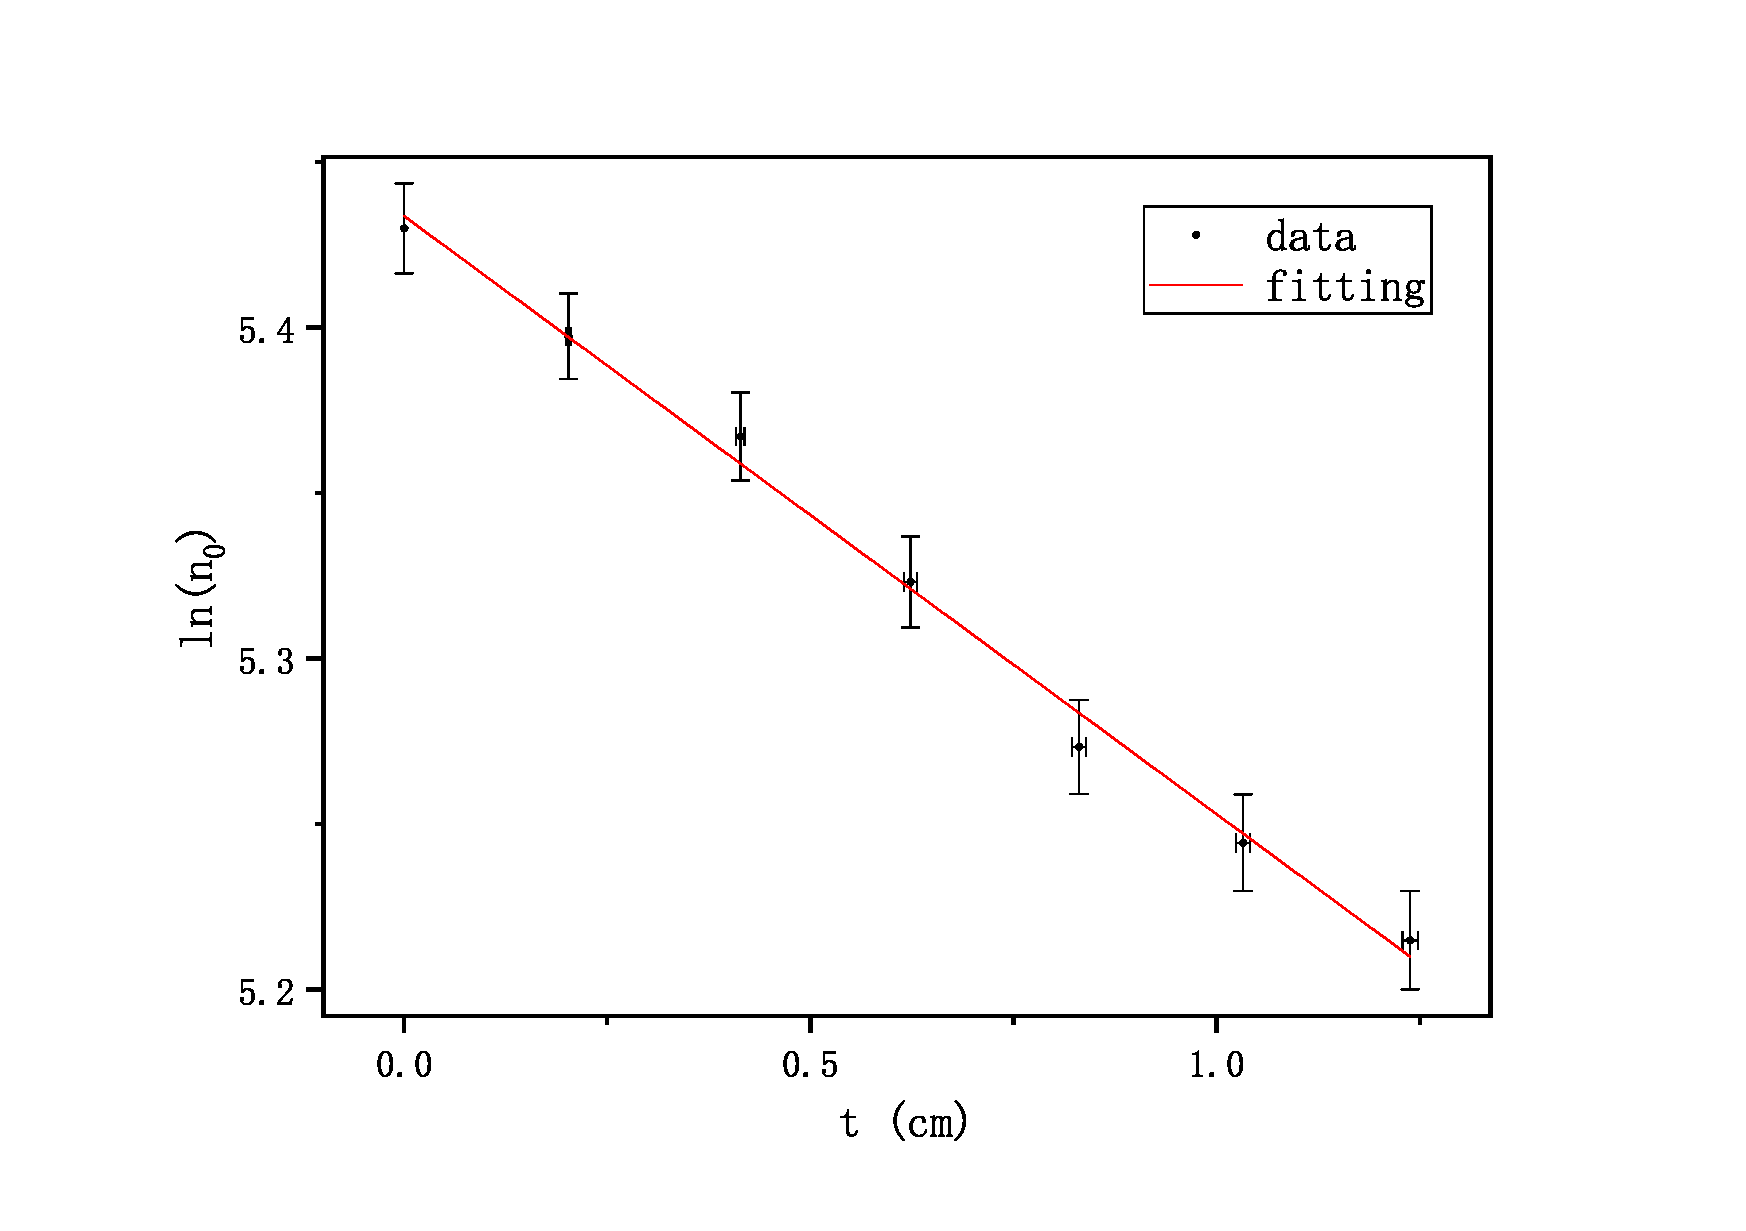
\includegraphics[width=0.9\linewidth]{lnn0-t.eps}
	\caption{$ \ln n_0-t $直线}
\end{figure}

\section{误差分析}
查阅相关资料得：$\rm \mu(Fe)=0.42cm^{-1} $，相对误差$\rm =(\mu(Fe)-\mu)/\mu(Fe)\times100\%=(57\pm2)\% $，分析误差来源主要有：
\begin{itemize}
	\item[1.]铁片厚度的误差，包括测量误差，以及未准直和铁片未放置水平带来的误差。
	
	\item[2.]计数误差，包括定标器的测量误差，以及未定标好带来的误差。
	
	\item[3.]实验条件未能契合原理要求带来的误差：(1)铁片上下表面有一层氧化物，它们对$ \gamma $射线的吸收系数与铁片不同；(2)空气和探头前的金属片也会吸收$ \gamma $射线；(3)探头有一定的面积。
\end{itemize}

\section{思考题}
\paragraph{1.什么叫$ \gamma $射线被吸收了？为什么说$ \gamma $射线通过物质时无射程概念？}
(1)$ \gamma $与物质发生相互作用(主要是光电效应、康普顿效应、电子对效应)偏离原来的传播方向即为被吸收。(2)$ \gamma $射线穿过物质时，$ \gamma $光子不会缓慢损失能量，而是直接与物质发生上述三种相互作用，发生大的能量转移，所以无射程概念。

\paragraph{2.物质对$ \gamma $射线的吸收系数与哪些因素有关？}
物质的种类(原子序数$ Z $)以及原子数密度、$ \gamma $射线的能量。

\section{实验总结}
通过本次实验，进一步了解了$ \gamma $射线与物质相互作用的特性，探究它在物质中的吸收规律并测量了物质的吸收系数，对$ \gamma $射线的了解更加深入。通过数据处理和分析，加强了数据处理能力以及Origin和\LaTeX{}的使用能力。总的来说，本次实验收获颇多。

\end{document}